\chapter{المفاعلات المستمرة والعمليات الصناعية}\label{ch:b2:continuous-reactors}

في المختبر يُجرى التفاعل في دورق: تُدخل الكواشف، ويُحرَّك الخليط ساعة،
ثم يُوقف التفاعل ويُعزل الناتج. أما المصنع الذي يصنع الناتج نفسه بآلاف
الأطنان فيعمل على نحو آخر. فمفاعله لا يفرغ أبدًا: تتدفق المتفاعلات من
طرف، وتخرج النواتج من الطرف الآخر، ليلًا ونهارًا، ولا يتغير التركيب في
داخله مع الزمن. فيحل سؤالان محل سؤال «كم من الوقت؟»: ما الحجم الذي يلزم
المفاعل لبلوغ \omterm{def:b2:continuous-reactors:conversion}{تحويل} معيّن، وكيف تُصرف حرارة التفاعل قبل أن تسخّن المفاعل
حتى يخرج عن السيطرة؟ يكتب هذا الفصل حصيلتي المادة والطاقة للمفاعلين
المستمرين المثاليين، الخزان المحرَّك والأنبوب، ويقارن بينهما، ويبيّن كيف
يمكن أن تكون للمفاعل عدة حالات ممكنة، إحداها جموح.

\begin{recall}
مجلد السنة الأولى: سرعة التفاعل، وقوانين السرعة والرتب، والقوانين المكاملة
في مفاعل مغلق (يُسمّى الآن \omterm{def:b2:continuous-reactors:reactors}{مفاعل دفعات})، وزمن نصف التفاعل، وقانون أرهينيوس
$k = A\,\mathrm e^{-E_a/RT}$، والتفاعلات المتتالية.
\Cref{ch:b2:reaction-enthalpy}: الحرارة المحررة عند ضغط ثابت؛
و\cref{ch:b2:equilibrium-shifts}: \omterm{def:b2:equilibrium-shifts:single-pass}{التحويل في مرور واحد}، وإعادة التدوير. ومن
الفيزياء: حصيلة نظام مفتوح في جريان مستقر (الداخل ناقص
الخارج يساوي المتراكم).
\end{recall}

\begin{omfigure}
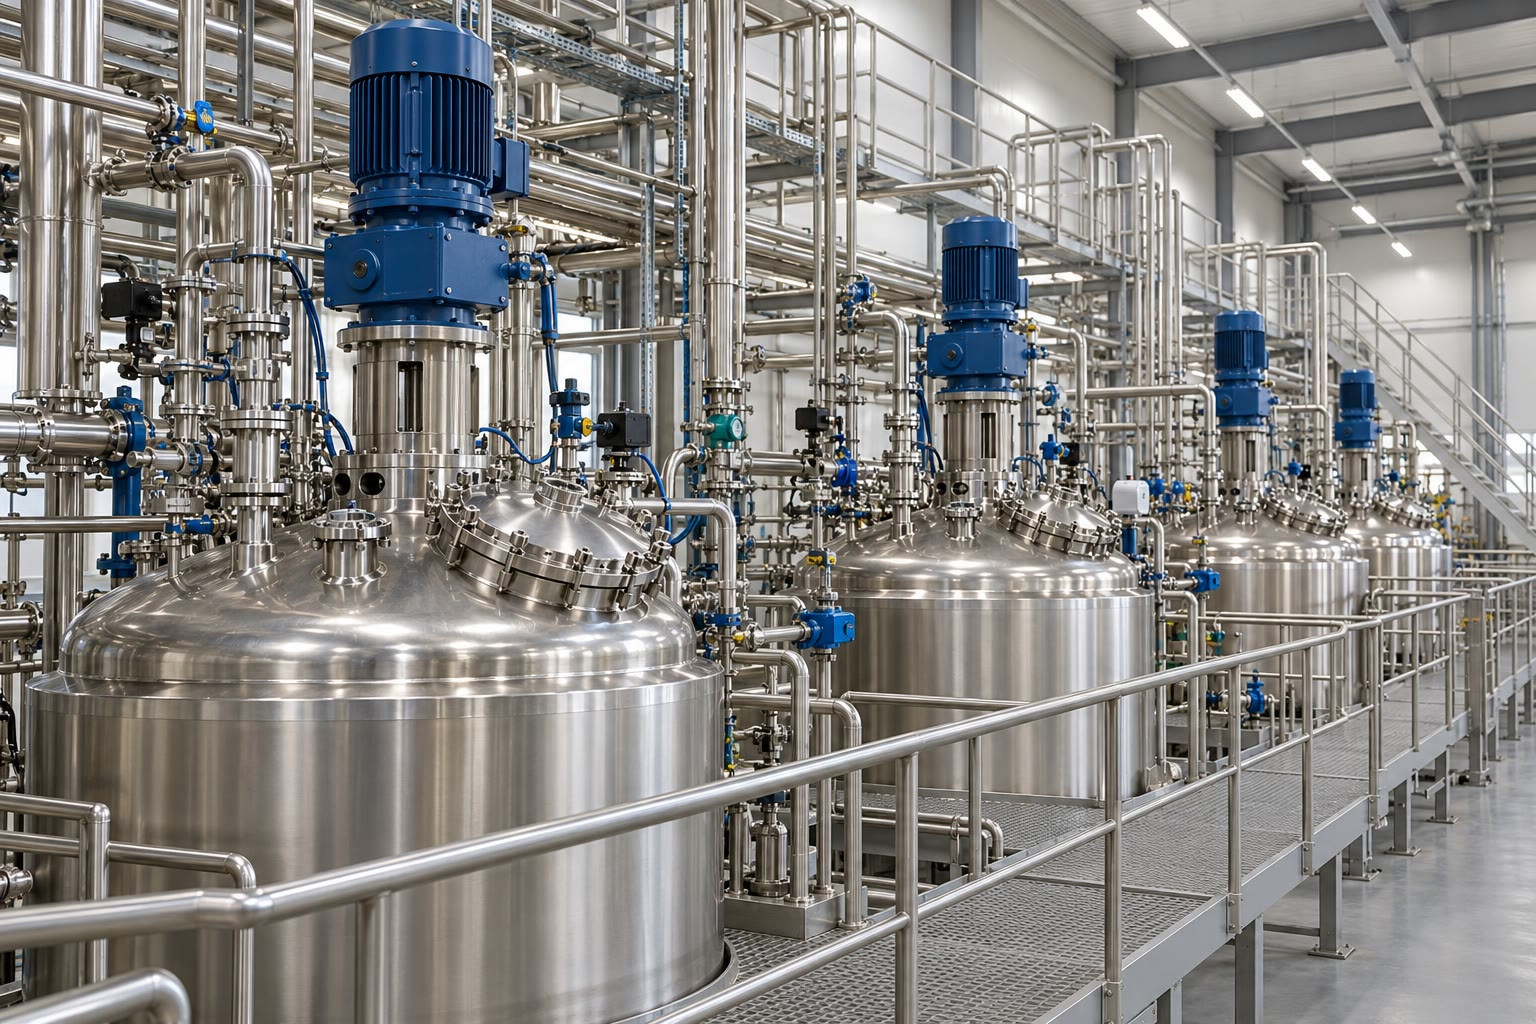
\includegraphics[width=0.6\linewidth]{images/book3/ai/b2-05-stirred-tanks.jpg}

{\small مفاعلات من نوع الخزان المحرَّك في مصنع كيميائي: يحمل كل وعاء محركه
وعلبة تروسه، ويهبط عمود المحرِّك في خليط التفاعل؛ وتجلب الأنابيب التغذيات
وتأخذ الناتج وماء التبريد.}
\end{omfigure}

\section{من مفاعل الدفعات إلى المفاعل المستمر}

\begin{definition}[أنواع المفاعلات]\label{def:b2:continuous-reactors:reactors}
\emph{مفاعل الدفعات}\index{مفاعل دفعات} وعاء مغلق يجري فيه
التفاعل دون دخول مادة أو خروجها. و\emph{المفاعل
المستمر}\index{مفاعل مستمر} يعبره جريان مستقر من المادة. ويُتخذ مفاعلان
مستمران مثاليان نموذجين:
\begin{itemize}
  \item \emph{مفاعل الخزان المحرَّك المستمر}\index{مفاعل الخزان المحرَّك المستمر}،
        وهو محرَّك تحريكًا جيدًا يجعل محتواه
        متجانسًا، ومن ثم مطابقًا للتيار الخارج منه؛
  \item \emph{مفاعل الجريان المكبسي}\index{مفاعل الجريان المكبسي}، وهو أنبوب
        يعبره المائع دون اختلاط على طول الجريان، فتتقدم كل شريحة من
        المائع كأنها مكبس وهي تتفاعل.
\end{itemize}
\end{definition}

يُقال إن \omterm{def:b2:continuous-reactors:reactors}{المفاعل المستمر} يعمل في \emph{تشغيل مستقر} حين لا يتغير شيء في
داخله مع الزمن: فالتدفقات ودرجات الحرارة والتراكيب في كل نقطة
ثابتة. ونعتبر تفاعلًا وحيدًا
$\mathrm A \to$ نواتج، وتغذية سائلة ذات كثافة ثابتة (فيكون
التدفق الحجمي $Q_v$ نفسه عند المدخل والمخرج)، تركيزها
$c_{A,0}$ عند المدخل.

\begin{definition}[زمن المكوث]\label{def:b2:continuous-reactors:residence-time}
\emph{زمن المكوث}\index{زمن المكوث} \omterm{def:b2:continuous-reactors:reactors}{لمفاعل مستمر} حجمه
$V$ يُغذّى بتدفق حجمي $Q_v$ هو $\tau = V/Q_v$: أي متوسط
الزمن الذي يقضيه حجم من المائع في داخله.
\end{definition}

\begin{definition}[التحويل]\label{def:b2:continuous-reactors:conversion}
\emph{تحويل}\index{تحويل} المتفاعل A هو $X = (F_{A,0} -
F_A)/F_{A,0}$، حيث $F_{A,0}$ و$F_A$ التدفقان الموليان للمتفاعل A
الداخل إلى المفاعل والخارج منه؛ وفي \omterm{def:b2:continuous-reactors:reactors}{مفاعل الدفعات}، $X = (n_{A,0} -
n_A)/n_{A,0}$. وعند كثافة ثابتة، $X = 1 - c_A/c_{A,0}$.
\end{definition}

يتعلق \omterm{def:b2:continuous-reactors:conversion}{التحويل} بمتفاعل واحد، وبمفاعل أو بمرور واحد؛ أما نسبة التقدم
النهائي في مجلد السنة الأولى فتتعلق بتفاعل وبمتفاعله
المحدِّد. ومن أجل تفاعل وحيد متفاعله المحدِّد هو A، تتطابق
الكميتان.

\begin{proposition}[مفاعل الدفعات]\label{prop:b2:continuous-reactors:batch}
في \omterm{def:b2:continuous-reactors:reactors}{مفاعل دفعات} ذي حجم ثابت، يبلغ تفاعل من الرتبة الأولى
\omterm{def:b2:continuous-reactors:conversion}{التحويل} $X = 1 - \mathrm e^{-kt}$ بعد الزمن $t$، ويبلغ تفاعل من الرتبة
الثانية بتركيزين ابتدائيين متساويين $c_0$ \omterm{def:b2:continuous-reactors:conversion}{التحويل} $X =
kc_0t/(1 + kc_0t)$.
\end{proposition}

\begin{proof}
هذه هي قوانين السرعة المكاملة في مجلد السنة الأولى، $c_A = c_{A,0}
\mathrm e^{-kt}$ و$1/c_A = 1/c_{A,0} + kt$، مكتوبة بواسطة $X = 1 -
c_A/c_{A,0}$.
\end{proof}

\section{مفاعل الخزان المحرَّك المستمر}

\begin{omfigure}
\begin{tikzpicture}[font=\small, >={Stealth}]
  % batch
  \pic[transform shape] at (0,0) {rbflask={0.6}{omDef!20}};
  \node[below] at (0,-0.15) {مفاعل دفعات};
  % CSTR
  \begin{scope}[xshift=4.2cm]
    \draw[thick, fill=omDef!15] (-1.2,0) rectangle (1.2,2.4);
    \draw[thick] (0,3.0) -- (0,0.5);
    \draw[thick, fill=gray!40] (-0.5,0.45) rectangle (0.5,0.6);
    \draw[thick, fill=gray!30] (-0.25,3.0) rectangle (0.25,3.35);
    \draw[->, thick, omDef] (-2.8,2.0) -- (-1.2,2.0) node[pos=0.0, above, anchor=south west, inner sep=1pt] {$Q_v$, $c_{A,0}$};
    \draw[->, thick, omThm] (1.2,0.3) -- (2.5,0.3) node[pos=1, below] {$Q_v$, $c_A$};
    \node[fill=omDef!15, inner sep=1pt] at (0.62,1.5) {$V$, $c_A$};
    \node[below] at (0,-0.15) {خزان محرَّك};
  \end{scope}
  % PFR
  \begin{scope}[xshift=8.4cm, yshift=1.0cm]
    \draw[thick, fill=omDef!10] (0,0) rectangle (4.2,0.7);
    \fill[omThm!25] (2.0,0) rectangle (2.35,0.7);
    \draw[thick] (2.0,0) -- (2.0,0.7) (2.35,0) -- (2.35,0.7);
    \node[above] at (2.17,0.75) {$\dd V$};
    \draw[->, thick, omDef] (-0.9,0.35) -- (0,0.35) node[pos=0, above] {$F_{A,0}$};
    \draw[->, thick, omThm] (4.2,0.35) -- (5.0,0.35) node[pos=1, above] {$F_A$};
    \node[below] at (1.0,0) {$F_A(V)$};
    \node[below] at (2.1,-1.15) {أنبوب جريان مكبسي};
  \end{scope}
\end{tikzpicture}

{\small المفاعلات المثالية الثلاثة. دورق دفعات؛ وخزان محرَّك محتواه المتجانس
هو محتوى التيار الخارج؛ وأنبوب يعبره جريان مكبسي،
ينخفض فيه تدفق A من شريحة إلى شريحة.}
\end{omfigure}

\begin{proposition}[حصيلة الخزان المحرَّك]\label{prop:b2:continuous-reactors:cstr-balance}
في التشغيل المستقر، يحقق خزان محرَّك حجمه $V$ يختفي فيه A
بالسرعة $r$ (مول لكل لتر ولكل ثانية)
\[
  F_{A,0} - F_A - rV = 0, \qquad\text{أي}\qquad c_{A,0} - c_A = r\,\tau ,
\]
وتُحسب السرعة عند تركيب المخرج ودرجة حرارته.
\end{proposition}

\begin{proof}
حصيلة A على الخزان خلال $\dd t$: الداخل، $F_{A,0}\dd t$،
ناقص الخارج، $F_A\dd t$، ناقص المتفاعل، $rV\dd t$، يساوي
التراكم، المنعدم في التشغيل المستقر. ولأن الخزان متجانس، تكون السرعة
واحدة في كل مكان ومساوية لسرعة التيار الخارج. نقسم على $Q_v$.
\end{proof}

\begin{theorem}[التحويل في خزان محرَّك]\label{thm:b2:continuous-reactors:cstr}
من أجل تفاعل من الرتبة الأولى، $X = \dfrac{k\tau}{1 + k\tau}$؛ ومن أجل تفاعل
من الرتبة الثانية بتركيزين متساويين $c_0$ للمتفاعلين في التغذية، يكون
$X$ الجذر الواقع في $[0, 1]$ للمعادلة $Da\,(1 - X)^2 = X$، مع $Da =
kc_0\tau$.
\end{theorem}

\begin{proof}
الرتبة 1: $r = kc_A$، ومنه $c_{A,0} - c_A = k\tau c_A$، $c_A = c_{A,0}/(1 + k\tau)$
و$X = 1 - 1/(1 + k\tau)$. الرتبة 2: $r = kc_A^2$ (يبقى التركيزان
متساويين)، $c_0X = k\tau c_0^2(1 - X)^2$.
\end{proof}

الزمرة اللابعدية $Da = k\tau$ (أو $kc_0\tau$)، أي عدد دامكولر، تقارن \omterm{def:b2:continuous-reactors:residence-time}{زمن
المكوث} بالمقياس الزمني للتفاعل:
وهي وحدها تحدد \omterm{def:b2:continuous-reactors:conversion}{التحويل}.

\begin{method}[تحديد أبعاد مفاعل]\label{met:b2:continuous-reactors:size-reactor}
\begin{enumerate}
  \item اكتب قانون السرعة \omterm{def:b2:continuous-reactors:conversion}{والتحويل} المطلوب $X$.
  \item من حصيلة المفاعل المختار، أوجد عدد دامكولر
        الذي يعطي $X$.
  \item استنتج $\tau$ من $Da$ ومن ثابت السرعة عند درجة حرارة
        التشغيل، و$V = \tau Q_v$ من التدفق المراد معالجته.
\end{enumerate}
\end{method}

\section{مفاعل الجريان المكبسي}

\begin{theorem}[التحويل في مفاعل جريان مكبسي]\label{thm:b2:continuous-reactors:pfr}
في التشغيل المستقر، يخضع تدفق A على طول أنبوب جريان مكبسي
للعلاقة $\dd F_A/\dd V = -r$. ومن أجل تفاعل من الرتبة الأولى يعطي ذلك $X = 1 -
\mathrm e^{-k\tau}$، ومن أجل تفاعل من الرتبة الثانية بتغذيتين متساويتين $X =
Da/(1 + Da)$: أي قوانين \omterm{def:b2:continuous-reactors:reactors}{مفاعل الدفعات}، مع \omterm{def:b2:continuous-reactors:residence-time}{زمن المكوث} في
مكان الزمن.
\end{theorem}

\begin{proof}
حصيلة A على الشريحة الواقعة بين $V$ و$V + \dd V$: $F_A(V) - F_A(V + \dd V)
- r\,\dd V = 0$، ومنه المعادلة التفاضلية. ومع $F_A = Q_vc_A$ 
و$\dd V = Q_v\,\dd t'$ (حيث $t'$ الزمن الذي قضته شريحة في الأنبوب)، تصير
$\dd c_A/\dd t' = -r$: فكل شريحة \omterm{def:b2:continuous-reactors:reactors}{مفاعل دفعات} صغير يبقى في
الأنبوب مدة $\tau$. وفصل المتغيرات من أجل $r = kc_A$ يعطي $c_A = c_{A,0}
\mathrm e^{-k\tau}$ عند المخرج؛ ومن أجل $r = kc_A^2$، $1/c_A - 1/c_0 = k\tau$.
\end{proof}

\begin{omfigure}
\begin{tikzpicture}
\begin{axis}[
  width=0.75\linewidth, height=6cm, xmin=0, xmax=10, ymin=0, ymax=1.05,
  axis x line=bottom, axis y line=left, xlabel={\foreignlanguage{arabic}{عدد دامكولر $k\tau$}},
  ylabel={\foreignlanguage{arabic}{التحويل $X$}}, tick label style={font=\small},
  label style={font=\small}, clip=false,
  legend style={font=\scriptsize, draw=none, at={(0.98,0.05)}, anchor=south east}]
\addplot[omThm, very thick] table[x=Da, y=pfr] {figdata/out/bachelor-2-reactors-a.dat};
\addplot[omProp, thick] table[x=Da, y=five] {figdata/out/bachelor-2-reactors-a.dat};
\addplot[omProp, thick, dashed] table[x=Da, y=two] {figdata/out/bachelor-2-reactors-a.dat};
\addplot[omDef, very thick] table[x=Da, y=cstr] {figdata/out/bachelor-2-reactors-a.dat};
\legend{{جريان مكبسي}, {5 خزانات على التوالي}, {خزانان على التوالي}, {خزان محرَّك واحد}}
\draw[dotted] (axis cs:2.303,0) -- (axis cs:2.303,0.9) -- (axis cs:9,0.9);
\fill[omThm] (axis cs:2.303,0.9) circle (1.4pt);
\fill[omDef] (axis cs:9,0.9) circle (1.4pt);
\end{axis}
\end{tikzpicture}

{\small \omterm{def:b2:continuous-reactors:conversion}{تحويل} تفاعل من الرتبة الأولى بدلالة $k\tau$ في المفاعلات
المثالية. ولتحويل قدره 90\,\% يحتاج أنبوب الجريان المكبسي إلى $k\tau = \ln 10 = 2.3$،
والخزان المحرَّك الواحد إلى $k\tau = 9$: أي أربعة أضعاف الحجم. والخزانات على التوالي
تقترب من الأنبوب.}
% (model curves, computed in figdata/bachelor-2/reactors.py)
\end{omfigure}

\begin{proposition}[خزان أم أنبوب]\label{prop:b2:continuous-reactors:compare}
من أجل كل سرعة تتزايد مع تركيز A (أي رتبة موجبة)، يبلغ \omterm{def:b2:continuous-reactors:reactors}{مفاعل الجريان
المكبسي} تحويلًا معيّنًا بحجم أصغر
من حجم الخزان المحرَّك.
\end{proposition}

\begin{proof}
من الحصيلتين، $\tau_{\text{خزان}} = c_{A,0}X/r(X)$ (السرعة عند تركيب
المخرج) و$\tau_{\text{أنبوب}} = c_{A,0}\int_0^X\dd X'/r(X')$. ولأن $r$
يتناقص حين يتزايد $X$، فإن $1/r(X') \leq 1/r(X)$ على $[0, X]$، فلا يتجاوز
التكامل $X/r(X)$. وبيانيًا، على مخطط $1/r$ بدلالة $X$، تكون $\tau$
الأنبوب المساحة تحت المنحنى، وتكون قيمتها للخزان مساحة المستطيل الذي
ارتفاعه $1/r(X)$ (الشكل أدناه). ومن أجل الرتبة 1: $\ln(1 + k\tau) \leq k\tau$، وهو
القول نفسه بصيغة أخرى.
\end{proof}

يعمل الخزان المحرَّك كله عند تركيز المخرج، وهو الأدنى في
النظام، ومن ثم عند السرعة الدنيا؛ أما الأنبوب فيستفيد من التراكيز
العالية قرب مدخله. ومزايا الخزان في مكان آخر: درجة حرارة متجانسة سهلة الضبط،
وتشغيل بسيط.

\begin{omfigure}
\begin{tikzpicture}
\begin{axis}[
  width=0.62\linewidth, height=5.6cm, xmin=0, xmax=1, ymin=0, ymax=22,
  axis x line=bottom, axis y line=left, xlabel={\foreignlanguage{arabic}{التحويل $X$}},
  ylabel={\shortstack{\foreignlanguage{arabic}{$1/r$ (بوحدات النموذج)}}}, tick label style={font=\small},
  label style={font=\small}, clip=false]
\fill[omDef!15] (axis cs:0,0) rectangle (axis cs:0.9,10);
\addplot[omThm, fill=omThm!20, draw=none, domain=0:0.9, samples=60] {1/(1-x)} \closedcycle;
\addplot[black, very thick] table[x=X, y=invr] {figdata/out/bachelor-2-reactors-c.dat};
\draw[omDef, thick] (axis cs:0,10) -- (axis cs:0.9,10) -- (axis cs:0.9,0);
\node[omDef, font=\scriptsize, anchor=south] at (axis cs:0.45,10.2) {\foreignlanguage{arabic}{خزان محرَّك: المستطيل، $\tau = 9$}};
\node[omThm, font=\scriptsize, anchor=west] (pf) at (axis cs:0.05,6.5) {\foreignlanguage{arabic}{جريان مكبسي: المساحة المظللة، $\tau = \ln 10$}};
\draw[omThm, ->] (axis cs:0.25,6.0) -- (axis cs:0.3,0.8);
\end{axis}
\end{tikzpicture}

{\small مخطط ليفنشبيل لتفاعل من الرتبة الأولى ($k = 1$، $c_{A,0} = 1$).
\omterm{def:b2:continuous-reactors:conversion}{لتحويل} قدره 90\,\% يحتاج الخزان المحرَّك إلى المستطيل كله، والجريان
المكبسي إلى المساحة المظللة تحت المنحنى فقط.}
% (model, computed in figdata/bachelor-2/reactors.py)
\end{omfigure}

\begin{proposition}[خزانات على التوالي]\label{prop:b2:continuous-reactors:cascade}
$N$ خزانًا محرَّكًا متساوية على التوالي، زمن مكوثها الكلي $\tau$، تحوّل
تفاعلًا من الرتبة الأولى إلى $X_N = 1 - (1 + k\tau/N)^{-N}$، وهو يتزايد مع
$N$ ويؤول إلى قيمة الجريان المكبسي $1 - \mathrm e^{-k\tau}$.
\end{proposition}

\begin{proof}
كل خزان يقسم التركيز على $1 + k\tau/N$. و$(1 +
k\tau/N)^{-N} = \exp[-N\ln(1 + k\tau/N)] \to \mathrm e^{-k\tau}$، لأن
$N\ln(1 + u/N) \to u$.
\end{proof}

\begin{definition}[الانتقائية]\label{def:b2:continuous-reactors:selectivity}
حين يمكن لمتفاعل أن يعطي عدة نواتج، تكون \emph{الانتقائية}\index{انتقائية}
نحو الناتج المرغوب B هي كمية B المتكوّنة مقسومة على كمية
المتفاعل المستهلكة (مضروبة في النسبة الستوكيومترية): فهي تقول كم مما
تفاعل سلك الطريق الصحيح.
\end{definition}

\begin{proposition}[وسيط في خزان وفي أنبوب]\label{prop:b2:continuous-reactors:consecutive}
من أجل تفاعلين متتاليين من الرتبة الأولى $\mathrm A \xrightarrow{k_1} \mathrm B
\xrightarrow{k_2} \mathrm C$، مع تغذية من A وحده، يكون تركيز B
عند المخرج أكبر ما يمكن من أجل $\tau = \ln(k_2/k_1)/(k_2 - k_1)$ في
مفاعل جريان مكبسي ومن أجل $\tau = 1/\sqrt{k_1k_2}$ في خزان محرَّك؛ والقيمة
العظمى أعلى في الأنبوب.
\end{proposition}

\begin{proof}
الأنبوب: قوانين الدفعات في مجلد السنة الأولى، $c_B = c_{A,0}\frac{k_1}{k_2 - k_1}
(\mathrm e^{-k_1\tau} - \mathrm e^{-k_2\tau})$، وقيمتها العظمى حيث تنعدم
المشتقة، $k_1\mathrm e^{-k_1\tau} = k_2\mathrm e^{-k_2\tau}$. الخزان: $c_A =
c_{A,0}/(1 + k_1\tau)$ وحصيلة B، $c_B = k_1\tau c_A - k_2\tau c_B$،
تعطي $c_B = c_{A,0}k_1\tau/[(1 + k_1\tau)(1 + k_2\tau)]$، التي تنعدم مشتقتها
حين $k_1k_2\tau^2 = 1$. أما مقارنة القيمتين العظميين فهي
\cref{exo:b2:continuous-reactors:10}.
\end{proof}

\section{الحصيلة الحرارية والسلامة}

\begin{definition}[الارتفاع الكظوم لدرجة الحرارة]\label{def:b2:continuous-reactors:adiabatic-rise}
\emph{الارتفاع الكظوم لدرجة الحرارة}\index{ارتفاع كظوم لدرجة الحرارة}
$\Delta T_{\text{كظوم}}$ لخليط متفاعل هو ارتفاع درجة الحرارة الذي
يطرأ عليه لو كان التفاعل تامًا ولم تُصرف أي حرارة.
\end{definition}

\begin{proposition}[الارتفاع الكظوم لخليط سائل]\label{prop:b2:continuous-reactors:adiabatic}
من أجل خليط كثافته $\rho$ وسعته الحرارية الكتلية $c_p$، يتفاعل فيه
المتفاعل A، بتركيز $c_{A,0}$، بأنتالبي
$\Delta_r H$ لكل مول من A، يكون ارتفاع درجة الحرارة عند \omterm{def:b2:continuous-reactors:conversion}{التحويل} $X$ دون
فقد للحرارة
\[
  \Delta T = \frac{(-\Delta_r H)\,c_{A,0}\,X}{\rho\,c_p}, \qquad
  \Delta T_{\text{كظوم}} = \frac{(-\Delta_r H)\,c_{A,0}}{\rho\,c_p} .
\]
\end{proposition}

\begin{proof}
من أجل وحدة الحجم، تسخّن الحرارة المحررة، $(-\Delta_r H)c_{A,0}X$،
كتلة $\rho$ سعتها الحرارية $c_p$ (المبدأ الأول عند ضغط ثابت، والمرحلتان
في \cref{prop:b2:reaction-enthalpy:flame}).
\end{proof}

الخليط المخفف آمن: بضع درجات من الارتفاع. أما الخليط المركّز الشديد
النشر للحرارة فقد يسخّن نفسه بمئات الكلفنات، بما يكفي لإغلاء
المذيب أو لإطلاق تفاعل آخر. والسرعة تزداد أسيًا مع
درجة الحرارة: فالحرارة تسرّع التفاعل، فيحرر الحرارة أسرع.

\begin{proposition}[الحالات المستقرة لخزان محرَّك مبرَّد]\label{prop:b2:continuous-reactors:steady-states}
من أجل خزان محرَّك تغذيته عند $T_0$، مبرَّد بغلاف عند $T_0$ جداء
معامل انتقال الحرارة فيه في المساحة $UA$، تكون درجات الحرارة
المستقرة الممكنة $T$ حلول المعادلة
\[
  \underbrace{\Delta T_{\text{كظوم}}\,X(T)}_{\text{الحرارة المولَّدة}} =
  \underbrace{(1 + \kappa)(T - T_0)}_{\text{الحرارة المصروفة}}, \qquad
  \kappa = \frac{UA}{Q_v\rho c_p},
\]
حيث $X(T) = k(T)\tau/(1 + k(T)\tau)$ لتفاعل من الرتبة الأولى. التوليد
منحنى على شكل S بدلالة $T$، والصرف مستقيم: فقد تكون هناك نقطة تقاطع
واحدة أو ثلاث.
\end{proposition}

\begin{proof}
حصيلة الطاقة للخزان في التشغيل المستقر، في وحدة الزمن: الحرارة
التي يحررها التفاعل، $(-\Delta_r H)F_{A,0}X$، تخرج مع التيار
الخارج، الذي يسخن من $T_0$ إلى $T$، $Q_v\rho c_p(T - T_0)$، وعبر
الغلاف، $UA(T - T_0)$. نقسم على $Q_v\rho c_p$. ومع قانون أرهينيوس
يرتفع $X(T)$ من 0 إلى 1 على مجال ضيق من درجات الحرارة: إنه حرف S.
\end{proof}

\begin{omfigure}
\begin{tikzpicture}
\begin{axis}[
  width=0.75\linewidth, height=6.2cm, xmin=300, xmax=470, ymin=0, ymax=250,
  axis x line=bottom, axis y line=left, xlabel={\foreignlanguage{arabic}{درجة حرارة الخزان $T$ \babelsublr{(K)}}},
  ylabel={\foreignlanguage{arabic}{الحرارة لكل وحدة تدفق \babelsublr{(K)}}}, tick label style={font=\small},
  label style={font=\small}, clip=true]
\addplot[omThm, very thick] table[x=T, y=gen] {figdata/out/bachelor-2-reactors-b.dat};
\addplot[omDef, very thick] table[x=T, y=rem] {figdata/out/bachelor-2-reactors-b.dat};
\fill[black] (axis cs:300.03,0.04) circle (2pt);
\fill[white, draw=black] (axis cs:390.4,135.6) circle (2pt);
\fill[black] (axis cs:429.6,194.4) circle (2pt);
\node[font=\scriptsize, anchor=north west, fill=white, inner sep=1pt] at (axis cs:318,58) {\foreignlanguage{arabic}{بارد، مستقر}}; \draw[black!60] (axis cs:301.5,2) -- (axis cs:318,52);
\node[font=\scriptsize, anchor=north west] at (axis cs:393,132) {غير مستقر};
\node[font=\scriptsize, anchor=south east] at (axis cs:426,197) {\foreignlanguage{arabic}{ساخن، مستقر}};
\node[omThm, font=\scriptsize, anchor=north west] at (axis cs:440,196) {المولَّدة};
\node[omDef, font=\scriptsize, anchor=south east] at (axis cs:452,232) {المصروفة};
\end{axis}
\end{tikzpicture}

{\small مخطط سيميونوف لخزان محرَّك مبرَّد (وسائط نموذجية). تلتقي
الحرارة المولَّدة (بالأحمر) والحرارة المصروفة (المستقيم الأزرق) ثلاث مرات. والحالة
الوسطى غير مستقرة: فإن سخن الخزان قليلًا غلب التوليد وجمح
إلى الحالة الساخنة؛ وإن برد قليلًا عاد إلى الحالة
الباردة.}
% (model, computed in figdata/bachelor-2/reactors.py)
\end{omfigure}

يُستنتج استقرار كل حالة من الميول: عند نقطة تقاطع يكون فيها مستقيم
الصرف أشد ميلًا من منحنى التوليد، يصرف ارتفاع صغير في درجة الحرارة
حرارة أكثر مما يولّد، فيعود الخزان إلى البرودة؛ وحيث يكون منحنى التوليد
أشد ميلًا، يغذي الارتفاع الصغير نفسه بنفسه. (والتحليل الدقيق يجعل
الحصائل المتعلقة بالزمن خطية؛ ونقبله
هنا.)

\begin{definition}[الجموح الحراري]\label{def:b2:continuous-reactors:runaway}
\emph{الجموح الحراري}\index{جموح حراري} هو الارتفاع المتسارع ذاتيًا
لدرجة حرارة خليط متفاعل يفوق فيه توليدُ الحرارة، المتزايد
أسيًا مع درجة الحرارة، صرفَها.
\end{definition}

\begin{method}[الحصيلة الحرارية لمفاعل]\label{met:b2:continuous-reactors:heat-balance}
\begin{enumerate}
  \item احسب \omterm{def:b2:continuous-reactors:adiabatic-rise}{الارتفاع الكظوم لدرجة الحرارة}: فإن كان بضعة كلفنات كان
        المفاعل آمنًا حراريًا.
  \item وإلا فاحسب حمل التبريد، $(-\Delta_r H)F_{A,0}X$ ناقص
        الحرارة التي يحملها التيار الخارج، وتحقق من أن الغلاف أو الملف
        قادر على صرفها.
  \item تحقق من استقرار نقطة التشغيل (الميول على مخطط
        سيميونوف)، ومما قد يحدث لو تعطل التبريد: أي درجة الحرارة
        القصوى المبلوغة، $T + \Delta T_{\text{كظوم}}(1 - X)$ من أجل
        المتفاعل الذي ما زال موجودًا.
\end{enumerate}
\end{method}

\section{من البروتوكول إلى المصنع}

التخليق الذي ينجح في دورق سعته \qty{1}{L} لا يُكبَّر ببساطة ألف
مرة. فالحجم، والحرارة المحررة معه، يكبران كمكعب البعد؛ والجدار، الذي
تخرج منه الحرارة، كمربعه. فالوعاء الأعرض بعشر مرات حجمه أكبر بألف مرة
لكن سطح تبريده أكبر بمئة مرة فقط: فالتفاعل الذي بقي فاترًا في الدورق قد يجمح
في الخزان. ولهذا تضيف الممارسة الصناعية الكاشف الأشد تفاعلًا
ببطء (فلا يستطيع التفاعل تحرير حرارة أكثر مما يتيحه الكاشف المضاف)، وتخفف،
وتبرد بملفات داخلية، أو تنتقل إلى مفاعلات مستمرة صغيرة الحجم،
يحدّ محتواها الصغير مما يمكن أن يسوء.

\omterm{def:b2:continuous-reactors:selectivity}{والانتقائية} هي الهمّ الآخر. فالمصنع لا يرمي ما لم
يتفاعل: بل يفصل الناتج ويعيد تدوير المتفاعلات، كما في حلقة
الأمونيا. ولذلك يمكنه أن يقبل تحويلًا متواضعًا في مرور واحد إذا كانت
\omterm{def:b2:continuous-reactors:selectivity}{الانتقائية} عالية، لأن كل ناتج ثانوي مادة أولية ضائعة ونفاية يجب
معالجتها.

\begin{inthelab}[خزان محرَّك على طاولة المختبر]
تُقاس حركية تفاعل معدّ لمصنع مستمر في مفاعل محرَّك صغير
تغذيه مضختان معايَرتان، مع خلية لقياس الموصلية
أو مطياف مباشر عند المخرج. وتغيير التدفق يغيّر $\tau$؛
والتركيز المستقر عند المخرج لكل $\tau$ يعطي السرعة مباشرة، بواسطة
الحصيلة $r = (c_{A,0} - c_A)/\tau$، دون أي مكاملة.
\end{inthelab}

\section{تمارين}

\begin{exercise}[$\star$]\label{exo:b2:continuous-reactors:1}
يُغذّى خزان محرَّك حجمه \qty{2.0}{m^3} بتدفق \qty{0.50}{L/s}. احسب زمن
مكوثه بالثواني وبالساعات.
\end{exercise}

\begin{exercise}[$\star$]\label{exo:b2:continuous-reactors:2}
لتفاعل من الرتبة الأولى $k = \qty{1.2e-3}{s^{-1}}$ عند درجة حرارة
التشغيل. احسب \omterm{def:b2:continuous-reactors:conversion}{التحويل} في خزان محرَّك وفي أنبوب جريان مكبسي
لهما \omterm{def:b2:continuous-reactors:residence-time}{زمن المكوث} نفسه، \qty{30}{min}.
\end{exercise}

\begin{exercise}[$\star$]\label{exo:b2:continuous-reactors:3}
ما \omterm{def:b2:continuous-reactors:residence-time}{زمن المكوث} في الجريان المكبسي الذي يعطي تحويلًا قدره 99\,\% لتفاعل من الرتبة الأولى
مع $k = \qty{0.020}{s^{-1}}$؟ وفي خزان محرَّك؟
\end{exercise}

\begin{exercise}[$\star$]\label{exo:b2:continuous-reactors:4}
محلول مائي بتركيز \qty{0.50}{mol/L} لمتفاعل يحرر تفاعله
\qty{-120}{kJ/mol} ($\rho = \qty{1.0}{kg/L}$، $c_p =
\qty{4.2}{J/(g.K)}$) يتفاعل تفاعلًا تامًا. احسب \omterm{def:b2:continuous-reactors:adiabatic-rise}{الارتفاع الكظوم لدرجة
الحرارة}. هل يكون تعطل التبريد خطرًا؟
\end{exercise}

\begin{exercise}[$\star\star$]\label{exo:b2:continuous-reactors:5}
من أجل تفاعل من الرتبة الثانية بتغذيتين متساويتين ($kc_0 = \qty{0.010}{s^{-1}}$)،
احسب \omterm{def:b2:continuous-reactors:residence-time}{زمن المكوث} اللازم \omterm{def:b2:continuous-reactors:conversion}{لتحويل} قدره 80\,\% في خزان محرَّك وفي أنبوب
جريان مكبسي. وقارن النسبة بنسبة تفاعل من الرتبة الأولى.
\end{exercise}

\begin{exercise}[$\star\star$]\label{exo:b2:continuous-reactors:6}
ثلاثة خزانات محرَّكة متساوية على التوالي، زمن مكوثها الكلي \qty{10}{min}،
تعالج تفاعلًا من الرتبة الأولى مع $k = \qty{0.50}{min^{-1}}$. احسب
\omterm{def:b2:continuous-reactors:conversion}{التحويل} وقارنه بخزان واحد وبأنبوب له \omterm{def:b2:continuous-reactors:residence-time}{زمن المكوث} الكلي
نفسه.
\end{exercise}

\begin{exercise}[$\star\star$]\label{exo:b2:continuous-reactors:7}
يحوّل خزان محرَّك 70\,\% من متفاعل (الرتبة الأولى). يُضاعَف التدفق.
ما \omterm{def:b2:continuous-reactors:conversion}{التحويل} الجديد؟ وبأي عامل يجب أن يكبر الحجم لاسترجاع
70\,\%؟
\end{exercise}

\begin{exercise}[$\star\star$]\label{exo:b2:continuous-reactors:8}
يعمل خزان حجمه \qty{5.0}{m^3} عند \qty{350}{K} بتغذية فيها
\qty{2.0}{mol/L} من المتفاعل بتدفق \qty{1.0}{L/s}، يُحوَّل منها 90\,\%، و$\Delta_r H
= \qty{-80}{kJ/mol}$، و$\rho c_p = \qty{4.0}{kJ/(L.K)}$، والتغذية عند \qty{330}{K}.
احسب الحرارة المحررة في الثانية، والحرارة التي يحملها التيار
الخارج، وحمل التبريد على الغلاف.
\end{exercise}

\begin{exercise}[$\star\star$]\label{exo:b2:continuous-reactors:9}
لدورق سعته \qty{1.0}{L} ومفاعل سعته \qty{1.0}{m^3} الشكل نفسه.
بأي عامل يُضرب الحجم، ومساحة الجدار، والنسبة بينهما؟ وفسّر لماذا قد
يجمح في المفاعل تفاعلٌ يسهل تبريده في الدورق.
\end{exercise}

\begin{exercise}[$\star\star\star$]\label{exo:b2:continuous-reactors:10}
من أجل $\mathrm A \to \mathrm B \to \mathrm C$ مع $k_1 = \qty{0.10}{min^{-1}}$
و$k_2 = \qty{0.050}{min^{-1}}$، احسب \omterm{def:b2:continuous-reactors:residence-time}{زمن المكوث} الأمثل والمردود
الأقصى من B في مفاعل جريان مكبسي وفي خزان محرَّك، وفسّر
لماذا يتفوق الأنبوب في حالة الوسيط.
\end{exercise}

\begin{exercise}[$\star\star\star$]\label{exo:b2:continuous-reactors:11}
مستعملًا مخطط سيميونوف في الفصل، صِف ما يحدث حين تُرفع
درجة حرارة سائل التبريد ببطء، ثم تُخفض ببطء من جديد: وبيّن أن
الخزان يقفز من الفرع البارد إلى الفرع الساخن عند درجة حرارة ويعود عند
أخرى (تخلّف).
\end{exercise}

\begin{exercise}[$\star\star\star$]\label{exo:b2:continuous-reactors:12}
يُشحن \omterm{def:b2:continuous-reactors:reactors}{مفاعل دفعات} بمتفاعل تركيزه \qty{2.0}{mol/L} ($\Delta_r H =
\qty{-100}{kJ/mol}$، $\rho c_p = \qty{4.0}{kJ/(L.K)}$) ويُسخَّن إلى
درجة حرارة التشغيل. ثم يتعطل التبريد عند \omterm{def:b2:continuous-reactors:conversion}{تحويل} قدره 25\,\%. احسب
درجة الحرارة التي يمكن أن يبلغها الخليط. وفي تشغيل نصف مستمر يُضاف
المتفاعل نفسه ببطء ويُستهلك كلما وصل، بحيث لا يوجد منه في أي لحظة أكثر من 5\,\%
من الشحنة دون تفاعل: ما الارتفاع في أسوأ الحالات الآن؟
\end{exercise}

\section{مسألة: الصابون في خزان}

\begin{problem}[{مسألة نهاية الأسبوع --- تصبّن إستر في خزان
محرَّك: الحركية، وتحديد الأبعاد لتحويل قدره 90\,\%، وبديلا الأنبوب
والسلسلة، والحصيلة الحرارية}]
\label{pb:b2:continuous-reactors:1}
يتصبّن إيثانوات الإيثيل بهيدروكسيد الصوديوم،
\ce{CH3COOC2H5 + OH- -> CH3COO- + C2H5OH}، وهو تفاعل من الرتبة الثانية (من
الرتبة الأولى بالنسبة إلى كل متفاعل). يعالج مصنع \qty{0.50}{L/s} من خليط
تركيزا الإستر والهيدروكسيد فيه عند المدخل كلاهما $c_0 =
\qty{0.10}{mol/L}$. خذ في هذه المسألة $k = \qty{0.11}{L/(mol.s)}$ عند
درجة حرارة التشغيل و$\Delta_r H = \qty{-55}{kJ/mol}$ (قيم مثبتة من أجل
التمرين)؛ وللخليط كثافة الماء وسعته الحرارية،
$\rho = \qty{997}{kg/m^3}$، $c_p = \qty{4.18}{kJ/(kg.K)}$.

\medskip
\noindent\textbf{الجزء الأول --- الحركية.}
\begin{enumerate}
  \item اكتب قانون السرعة. لماذا يبقى التركيزان متساويين؟
  \item كم يستغرق \omterm{def:b2:continuous-reactors:conversion}{تحويل} قدره 90\,\% في دورق دفعات؟
  \item احسب زمن نصف التفاعل في الدورق. لماذا يتعلق بالتركيز $c_0$؟
  \item اكتب عدد دامكولر للتفاعل من أجل زمن مكوث $\tau$.
\end{enumerate}

\medskip
\noindent\textbf{الجزء الثاني --- خزان محرَّك واحد.}
\begin{enumerate}[resume]
  \item اكتب حصيلة الإستر في الخزان في التشغيل المستقر.
  \item بيّن أن $Da\,(1 - X)^2 = X$.
  \item احسب عدد دامكولر اللازم من أجل $X = 0.90$.
  \item احسب \omterm{def:b2:continuous-reactors:residence-time}{زمن المكوث}.
  \item احسب حجم الخزان.
  \item ما التركيز الذي «يراه» التفاعل في كل مكان من الخزان،
        ولماذا يكون الخزان بهذا الكبر؟
\end{enumerate}

\medskip
\noindent\textbf{الجزء الثالث --- أنبوب، وسلسلة.}
\begin{enumerate}[resume]
  \item احسب عدد دامكولر وحجم أنبوب جريان مكبسي يؤدي
        المهمة نفسها.
  \item احسب نسبة الحجمين.
  \item ثلاثة خزانات متساوية على التوالي: اكتب العلاقة بين تركيزي المخرج
        لخزانين متتاليين.
  \item الحجم الكلي للخزانات الثلاثة الذي يعطي 90\,\% هو
        \qty{0.85}{m^3}. تحقق من ذلك بحساب التركيز الخارج من كل
        خزان.
  \item أي ترتيب كنت ستبني، ولماذا قد يبقى الخزان الواحد
        مفضَّلًا مع ذلك؟
\end{enumerate}

\medskip
\noindent\textbf{الجزء الرابع --- الحرارة.}
\begin{enumerate}[resume]
  \item احسب الارتفاع الكظوم لدرجة حرارة الخليط.
  \item احسب الحرارة المحررة في الثانية في الخزان.
  \item هل يلزم التبريد؟ وهل الجموح ممكن؟
  \item ما الذي يتغير لخليط يُغذّى بتركيز \qty{2.0}{mol/L}؟
  \item احسب كتلة إيثانوات الصوديوم المنتجة في اليوم.
  \item إذا أُجري التفاعل عند درجة حرارة أعلى، كيف يتغير حجم الخزان،
        وما الثمن؟
  \item اذكر حجم الخزان المحرَّك الواحد الذي يحوّل 90\,\% من
        الإستر بهذه التغذية.
\end{enumerate}
\end{problem}
